%!TEX root = ../template.tex
%%%%%%%%%%%%%%%%%%%%%%%%%%%%%%%%%%%%%%%%%%%%%%%%%%%%%%%%%%%%%%%%%%%
%% chapter1.tex
%% NOVA thesis document file
%%
%% Chapter with introduction
%%%%%%%%%%%%%%%%%%%%%%%%%%%%%%%%%%%%%%%%%%%%%%%%%%%%%%%%%%%%%%%%%%%

\typeout{NT FILE chapter2.tex}%

\chapter{State of the Art}
\label{cha:State of the Art}

\prependtographicspath{{Chapters/Figures/Covers/}}

This chapter is divided into several sections. The first one gives an introduction to

\section{Identity Governance and Administration (IGA)}
\label{sec:IGA}

Identity Governance and Administration (IGA) plays a pivotal role in modern IT operations, enabling organizations to effectively manage user identities and access across the enterprise. It combines two critical components: Identity Governance and Identity Administration.

    Identity Governance focuses on:
        Visibility: Providing insights into user identities and access privileges.
        Segregation of Duties: Ensuring that conflicting roles are separated to prevent misuse.
        Role Management: Defining and assigning roles for efficient access control.
        Attestation: Regularly reviewing and validating access rights.
        Analytics and Reporting: Leveraging data for informed decision-making.

    Identity Administration encompasses:
        Account Administration: Managing user accounts and their attributes.
        Credentials Administration: Handling passwords, tokens, and other authentication factors.
        User and Device Provisioning: Automating user access throughout their lifecycle.
        Managing Entitlements: Controlling permissions and authorizations.


\subsection{Definition and Purpose}
\label{sec:Template}

Explain what IGA is: Identity Governance and Administration (IGA) is a set of policies and practices that enable organizations to manage and secure digital identities for users, applications, and data. Highlight its purpose: IGA helps balance the need to provide automated access to technology assets while managing security and compliance risks

\subsection{Components of IGA}
\label{sec:Template}

Identity Lifecycle Management: Covers user provisioning, deprovisioning, and modification of access rights throughout an individual’s lifecycle within an organization. Access Governance: Focuses on defining and enforcing policies related to access control, segregation of duties, and entitlement management. Access Administration: Involves managing user access requests, approvals, and access reviews. Role-Based Access Control (RBAC): Describes how roles are defined and assigned to users based on their job responsibilities. Policy Enforcement and Compliance: Ensures adherence to security policies, regulations (such as SOX, HIPAA, and GDPR), and audit requirements.

\subsection{Challenges and Considerations}
\label{sec:Template}

Complexity: IGA implementations can be intricate due to diverse user populations, applications, and data sources. Integration: Integrating IGA with existing systems and applications can be challenging. Scalability: As organizations grow, scalability becomes crucial. User Experience: Balancing security with a positive user experience is essential.

\section{Netwrix Usercube}
\label{sec:Template}

Netwrix Usercube is a product that is now part of Netwrix1. It is a comprehensive identity and access management solution. Netwrix Usercube enables organizations of all sizes to enhance their security and compliance posture by ensuring that access permissions are granted only to those who need them. It can automate onboarding and offboarding processes, easing the compliance burden.

\subsection{REFId}
\label{sec:Template}



\subsection{Ghab}
\label{sec:Template}

\subsection{Configuration}
\label{sec:Template}

A Usercube configuration is a set of XML files edited according the Usercube schema. The recommendations part of this section explains how to set up an editing environment for the configuration. Regardless of the editing space, the configuration persists in the Usercube database. It's this stored configuration that is used at runtime. The Deploy configuration tool is used to import a new version of the configuration (from the XML files set). The Export configuration tool can be used to export the current configuration (to a XML files set). The Usercube project's integration cycle consists in developing a configuration by successive imports in a test instance.

The XML configuration schema shows some similarities with the database schema but they are not the same.

\begin{figure}[htbp]
  \centering
  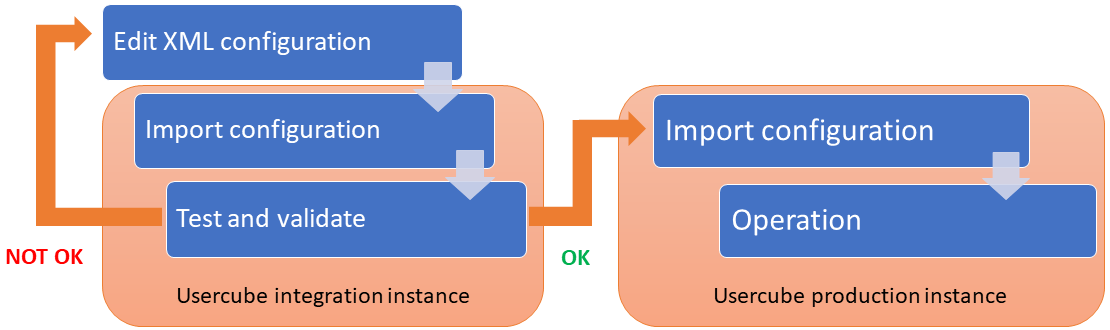
\includegraphics[width=5in]{configurationCycle}
  \caption{Usercube's configuration Cycle}
  \label{fig:configurationCycle}
\end{figure}

\subsection{Testing}
\label{sec:Template}

for testing we have different enviroments running in virtual machines. we deploy the new configuration to a testing instance and check if there is initial erros. Then the functional team is the one responsible to test the developments. After the test is done they send us back the ticket and then we save our code to build the next mep

\subsection{Deployment}
\label{sec:Template}

Deploy a local XML configuration by using the Deploy-Configuration executable and declaring at least: the configuration directory; the connection string of the database.

\section{Software Quality}
\label{sec:Template}

\subsection{Reverse Engineering}
\label{sec:Development models}

Reverse Engineering
 Involves analysing a subject system to determine its
components and relationship between them
 Involves creation of alternative representations of the
system, usually at a higher level of abstraction
 Does not involve changing or replicating system
 Only concerned with an examination of the system
 Can occur at any stage in s/w develop. life cycle

\subsection{Development models}
\label{sec:Development models}

\subsection{Lehman’s laws of software evolution}
\label{sec:Lehman}

The Lehman Laws of S/w evolution and S/w
development process models address different aspects
of the software development life cycle
 However, they are related in the sense that both
provide insights into the challenges and dynamics of
software development over time
 S/w development process models define ways in which
S/w projects are planned, executed, and controlled
 The Lehman Laws:
 Describe the evolution of S/w
 Suggest that S/w must continually evolve to remain useful

\subsection{Refactoring}
\label{sec:Refactoring}

\cite{fowler2018refactoring}
Martin Fowler [Fow99]: "a disciplined technique for restructuring an existing body of code, altering its internal structure without changing its external behaviour." William Wake [Wak04]: "Refactoring is the art of improving the design of existing code. Refactoring provides us with ways to recognize problematic code and gives us recipes for improving it."


\section{Related Work}
\label{sec:Template}